\section{Beginner friendly programming}
A lot of programming languages can be difficult to use for children and users with little to no experience in programming, as they are not used to the large amount of symbols, the logic behind control flow statements, and the even larger amount of keywords.

This chapter will therefore examine some of the characteristics that are needed for a language to be beginner friendly, both in terms of language design, but also in terms of what kind of, if any, Integrated Development Environment (IDE) should be provided with the language compiler.
An obvious example of an easy-to-learn for beginners language could be Scratch\cite{scratch}, which has an online IDE and compiler on one page. A great part of the success of Scratch comes from exactly that - the integrated IDE/compiler - which is incredibly easy for a kid to use.
Some widely used programming languages are not as beginner friendly as Scratch. Take for example this piece of code in Scheme:
\begin{figure}[H]
    \centering
    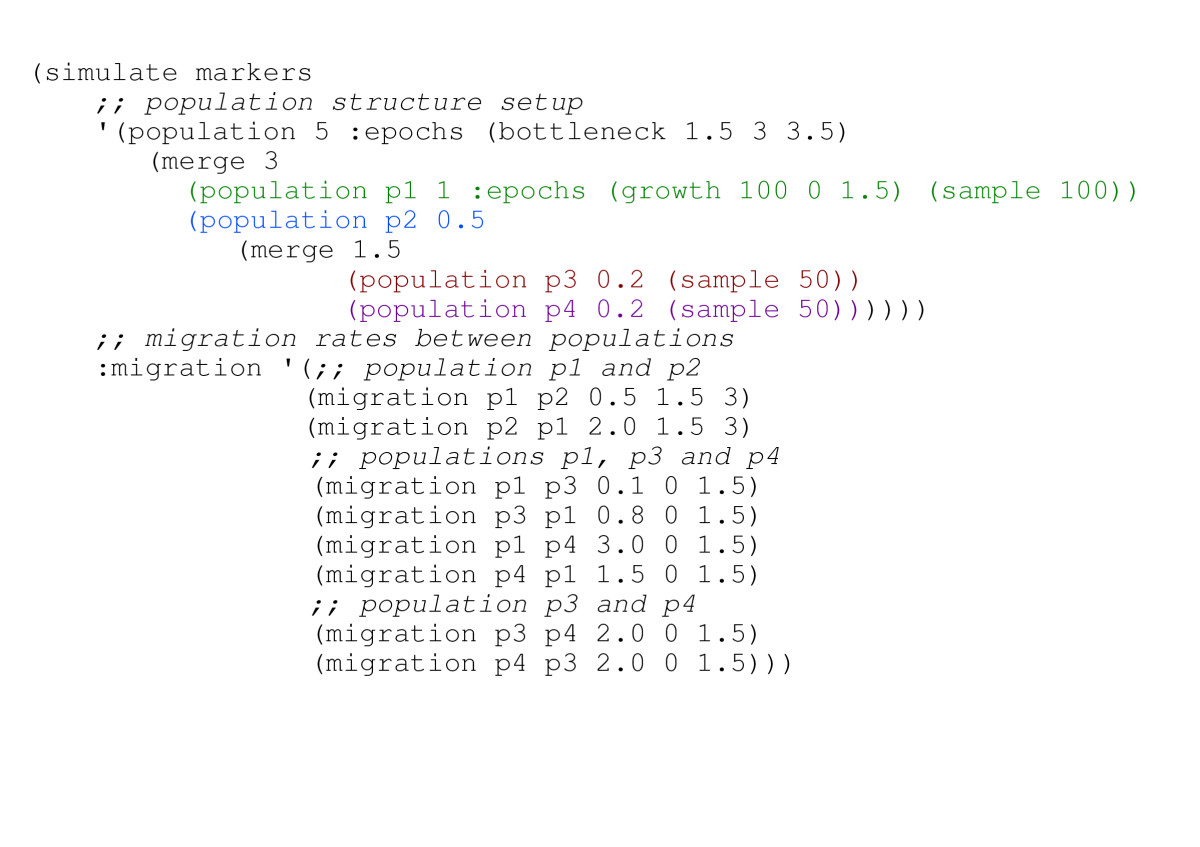
\includegraphics{resources/Images/schemes***.png}
    \caption{This example is supposed to function like a basic for-loop. It does something ten times.}\cite{Schemeexample}\label{fig:schemestuff}
\end{figure}

To the untrained eye, this will seem confusing. The keywords are not inherently easy to understand, and there are numbers/other symbols dispersed all over the code. Furthermore, the amount of parenthesis can easily confuse the user, as it is not clear which parenthesis belongs together, or even why they are there in the first place.

\subsection{Beginner friendly language design}
When making a language beginner friendly, there are a couple of things that should be taken into account. This section talks about the importance of keywords, dynamic and static typing, syntax structure, and type simplicity.
\subsubsection{Keywords}
The meaning (semantics) of a keyword should be readily seen, and intuitive when it is initially looked at. For example, the \textit{namespace} keyword in C\# can be used to declare a scope which can contain a collection of related objects. The objects could for example all belong to the same application, or maybe the same framework. It can be compared to sets in the mathematical fields, which is a collection of related symbols. Namespaces are a very common concept within programming and other computer related fields, but outside that, it is not really widely used or understood. Young users of programming languages will probably not have encountered the word before, and as such, it will contribute to the confusion of learning a new language. If instead of "namespace", something like "scope" or "set" had been used. It would help young users, or users new to programming in general to not be confused when initially learning the language.


\subsubsection{Dynamic and static typing}
Dynamic or static typing is very important for the readability of a language It is therefore important to make the right choice for new users. 
\\Dynamic typing means that a keyword like \textit{var} can be used in C\#, which allows the actual type of a variable to be determined at runtime. This can lead to a lot of confusion when type conversion exceptions are suddenly thrown during execution, because the user realistically has no idea what type of variable actually is in the variable. The upside is that it takes less time to write in this language, as the programmer does not have to think about what type the programmer wants something to be, and what representation of it the programmer wants to use. 
\\Static typing means that the programmer has to use the explicit type they want a variable to be when you are declaring it. This will usually lead to less confusion for inexperienced programmers, as they have to think about what they want a variable to be, and not just remember it based on what they do to that variable. This can however lead to confusing problems when converting between similar types, as for example in c\#, where there are multiple types for number-representation, such as: int, double and decimal. Some conversions between these are allowed, and others are not, which can lead to extra work and confusion when a type suddenly will not fit the input the programmer is giving it.

A language for beginners has to be clear and readable, and this is the main reason that static typing is better for beginners than dynamic typing. If the language is static, the beginner will not have unforeseen conversion errors, or variables that get the wrong input. Of course, cases as the one with multiple representations of numbers in c\# has to be avoided when using static typing. 


\subsubsection{Syntax structure}
When designing a syntax structure that is easy to read for beginners, simplicity is not the main focus, but rather readability. For example in Pascal, all variables has to be declared in the beginning of a function - or procedure as it is called in Pascal:

\lstset{language=[Sharp]C}  
\begin{figure}[H]
\centering
\begin{lstlisting}
procedure DoSomething; 
 var 
  x : Tsome_type;
  y : Tsome_otherType;
  z : Tsome_otherOthertype;
 begin
 if (x > y) then
      z := x
   
   else
      z := x;
   z := z;
 end;
\end{lstlisting}
\caption{Pascal local variable declaration.}\cite{pascalvar}
\label{fig:pascalvar}
\end{figure}
This can lead to somewhat unreadable code, because as it is read, each time a variable is encountered the reader has to go up and look at what kind of variable it is. The upside is that there can never be any doubt about where a variable is declared. A beginner might have a hard time remembering what types all his variables are, and having to go up and look might make it harder to read. 
\\Instead of doing it like in Pascal, it could be done like in Java, which allows variable declaration anywhere:
\lstset{language=[Sharp]C}  
\begin{figure}[H]
\centering
\begin{lstlisting}
public void SomeMethod(){

    int x = 0;
    x = x + 1;
    int y = 100;
    
    public void SomeOtherMethod();
    
    int z = 12;
    x = y+z+x;
    
    public void SomeOtherMethod();
}
\end{lstlisting}
\caption{Pascal local variable declaration.}
\label{fig:javavar}
\end{figure}
This allows variables to be declared where they are needed, and as such, it can improve the readability of the language. The downside of this is that when reading a method, the reader might have to look for a while to find a variable, if it is not properly placed closely to where it is used. 

\subsubsection{Type simplicity}
Keeping the types relatively simple is good for beginners, but only if the meaning of the type is also kept clear. For example, the meaning of \textit{char} in C is relatively clear, but the meaning of something like \textit{struct} is not. \textit{Struct} in itself is rather unintuitive.
So to be usable in a beginner friendly language, types should preferably be kept simple, and without too many different uses. It should not be presumed that beginners inherently know anything about the different constructs in programming. The meaning of a given type needs to be discernible from the type name.
\newpage
\subsection{Beginner friendly tools}
As a beginner, one of the most daunting tasks can be choosing the development environment in which to write code. In some languages, this is taken care of for you. For example in Scratch\cite{scratch}, where the only way to actually "write" in the language is through their website, with a visually based way of defining a program. 
If a beginner was to, for example, start in C\#\cite{CSHARP} and by extension use visual studio, it could be a very confusing experience. Visual studio has a mess of options, toolbars, windows and the like:
\begin{figure}[H]
    \centering
    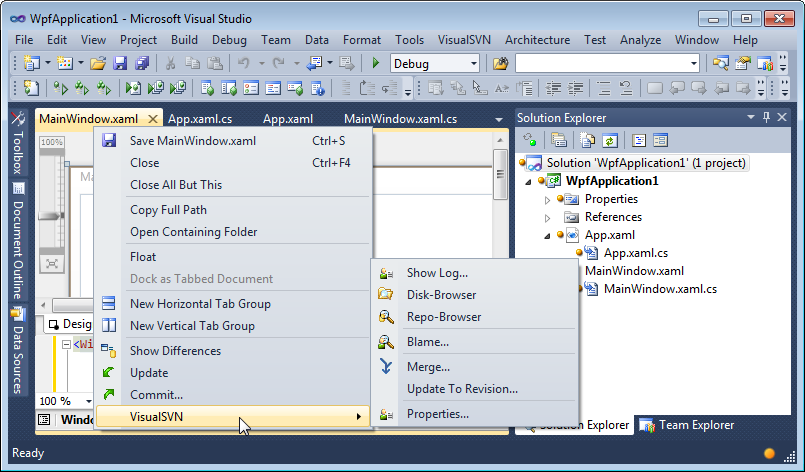
\includegraphics[scale=0.5]{resources/Images/vsclutter.png}
    \caption{Visual Studio clutter}
    \label{fig:vsclutter}
\end{figure}

This is hard to understand without some knowledge of programming beforehand. Therefore, it is useful for a beginner friendly programming language to have some kind of user friendly Interactive Development Environment (IDE) to let the user program in. Otherwise, it is going to be difficult for beginners to get started with programming in the language.
To summarize, it is important that the readability of the language is great when designing for beginners and kids. A more verbose syntax should be preferred over a clean and simple one, like in C\#\cite{CSHARP}, to make the writing of the language closer to actually writing a story, rather than programming a computer to do tasks. Types and keywords have to be intuitive in their use, and the complexity of any given type or keyword cannot be too great, or the readability will suffer from it. Furthermore, the medium in which the language is written is important. A user friendly IDE is paramount to help beginners getting started in a beginner friendly language.